\chapter{Ayalxrfna sUtarx}

\vskip -20pt

kirx.~sha. {\rm 1706} riMda {\rm 1783}ra. avadhiyalilxdadx sivxjalAyxRMDfna sherxVSaThx gaNitajacnx Ayalxrfna koDuge gaNitashAsatxrXkekx apAra. sumAru {\rm 900} saMshoVdhanA leVKanagaLanunx baredidAdxne. laGu gaNakada sidAdhxMtavanunx samapaRkavAda riVtiyalilx tiLisidAdxne.

$\sqrt{-1}$ eMbudakekx $i$ eMba cihenxyanunx koTuTx adanunx GAtavAgi $e^x$ eMdu modalu upayoVgisi kalapxnA saMKeyxyanunx parxcArakekx taMdavanu.

bahumuKa Gana matutx jAlAkaqtiya bagegx Ayalxrfna sUtarx bahaLa pArxmuKayx\-vAdudu.

oMdu bahumuKa Ganadalilx $V$ shaqMgagaLanUnx, $F$ muKagaLanUnx matutx $E$ aMcugaLanUnx sUcisidare Aga $V+F=E+2$ Aguvudu eMdu tiLisidavanu. 

keVvala {\rm 5} karxma GanAkaqtigaLu sAdhayx avugaLeV
\begin{enumerate}
\item[{\rm 1)}] karxma catuSaPxlaka (catumuRKa Gana)
\item[{\rm 2)}] karxma SaSaThxPalaka (SaNumxKa Gana)
\item[{\rm 3)}] karxma aSaTxPalaka (aSaTxmuKa Gana)
\item[{\rm 4)}] karxma dAvxdashaPalaka (dAvxdashamuKa Gana)
\item[{\rm 5)}] karxma viMshatiPalaka (viMshatimuKa Gana)
\end{enumerate}

\newpage
\phantom{a}

\vskip -0.7cm

udAharaNege karxma aSaTxPalaka (SaNumxKa Gana)dalilx \quad $V=8$, \quad $F=6$ matutx $E=12$
\begin{align*}
\therefore \;\; 8+6 &=12+2\\
14 &=14
\end{align*}

$V+F=E+2$ eMba Ayalxrfna sUtarx meVle tiLisida {\rm 5} karxma GanAkaqtigaLige mAtarx anavxyisutatxde.

bahu PalakagaLalilx avugaLa mUlaka hAduhoVguva suraMgagaLidadxre, I sUtarx anavxyisuvudilalx.

udAharaNege: TeYrinoLagiruva gALi tuMbida TUyxbf iruva hAge.
\begin{figure}[H]
\centering
\includegraphics{src/figures/m-147.eps}
\end{figure}

oMdu jAlAkaqtiyalilx $N$ saMpAta biMdugaLa {\rm (node)} saMKeyx, $A$ kaMsagaLa saMKeyx matutx $R$ samatalavanunx valayagaLanAnxgi viBAgisuva saMKeyxyAgidAdxga.

$N+R=A+2$ eMdu tiLisidAdxne. 

udAharaNege:
\begin{figure}[H]
\begin{minipage}[c]{4cm}
\centering
\includegraphics{src/figures/m_149.eps}
\end{minipage}
\qquad\qquad 
\begin{minipage}[c]{4cm}
\begin{gather*}
N = 5, \; R=5, \; A = 8, \\
5+5 = 8+2\\
10 = 10
\end{gather*}
\end{minipage}
\end{figure}

koVnisf bagfRna ELu seVtuvegaLa samaseyxge parihAra niVDiruvudu Ayalxrfna hesarinalilx parxKAyxtiyAgide.

aSeTxV alalx Ayalxrfna ELu seVtuveya samaseyxya vishelxVSaNeyu gaNitashAsatxrXda nUtana vidhAnavAda ToVpoVlajige nAMdiyAyitu.

{\rm 1783} ralilx liyonADoR Ayalxrf mAyAcwkagaLa racaneyalilx toDagidAdxga sUDoku anunx shoVdhisida eMdu tiLidubaMdide.

